\chapter{Research}%
\label{research}

\section{Theory}
% Brief explanation of why we needed to do so much research, as well
% as why it is so important for our style of project
% i.e. Exploratory Software

\subsection{StarCraft II}
% What is StarCraft II?

% Issues with StarCraft II
% Potentially, some of this can be moved to the implementation
% chapter too.
A game of StarCraft II includes many challenges for a player in terms of complexity.
The game state can be comprised of thousands of different aspects that could represent
important information for the player. In order for the agent to be able to act,
it must be given an input, stimulus of some form, to evaluate and then proceed with
taking an action. This makes the game ideal for an unsupervised learning environment.

The environment is broken into states. Each state represents information about
the game at a given moment.  This is then fed into the neural network and
returns a value outcome of what the optimal action to be taken would be.  A
different approach would be to use a Q-learning algorithm with a table format
for storing actions and values.  The main difficulty would be the size of the
given table.  As more actions are introduced the size of the table would
increase and new values would need to be optimized for the given cells.  Using
a neural network, this issue can be avoided by adding new weights and nodes to
the network.

\subsection{Q-Learning Table}

Q-Learning is a reinforcement learning algorithm
that uses a tabular approach to state action pairs. Q-Learning is an off-policy
method which gives the agent the ability to randomly select actions in a given
state without affecting the updated value of the state action pair. It requires:

\begin{itemize}
    \item State: A representation of the environment the agent is in.
    \item Action: An action that may move the agent
        from one state to the next or keep it in the same state.
\end{itemize}

The agent is given a state of the world and checks the lookup table for which
action would have the highest value in that state. The agent then executes that
action, before checking the table again for the new state. Upon executing an action the
agent may be given a reward, a value that dictates whether the action taken was
favourable or incorrect. The table can be updated through a real-time learning
or at the end of an episode. An episode represents an entire list of states and
actions taken to reach the end, usually by having a terminal state. The table
is updated using the Q-Learning equation.

% Add more info about how q learning works and the equation it uses

\subsection{Neural Networks}

Neural networks takes inspiration from the biological neurons that
are present in the brain, similar to how genetic learning
algorithms take inspiration from the physical process of evolution
and mutation\cite{goldberg2006genetic}.

Broadly, a Neural Network is a model that estimates a function $f$.
It does this by using a set of weights, and input neurons. A neuron
can be thought of some model that given a number of inputs, gives
an output which is some weighted sum of the inputs.

A given network can have any number of neurons, connected in a number
of different ways. Normally, neurons are arranged into layers, which
are sets of neurons who are all receiving from a given input, be
that an outside source, or a different layer of neurons. An explanation of
these layers will be given later. The communication
between the neurons is done by using the aforementioned weights, where
$w_{ij}$ denotes the weight between neurons $i$ and $j$. Depending on the
style of the network, there may be restrictions on the values of these
weights, and it is also possible that $w_{ij} \ne w_{ji}$.

For a value to be passed through the network, it is given as input to an input
layer, where it is then multiplied by the associated weights of the neuron the
value entered on, perhaps with the use of an associated activation function.  A
common activation function is the Rectified Linear Unit
(RELU)\cite{Nair:2010:RLU:3104322.3104425}, which works by taking the maximum
of two values as follows:

\begin{align}
    f(x) = \max(0, x)
\end{align}

where $x$ is the input value to the activation function.

For an average network, the layout of the layers is an input layer,
followed by a number of hidden layers, and finally an output layer. Usually
these layers are fully-connected, which means there every neuron in each
layer is connected to  every neuron in the following layer, but
there is no connections between neurons of the layer. An example of this
is shown in Figure~\ref{fig:common_layout}.

\begin{figure}
    \centering
    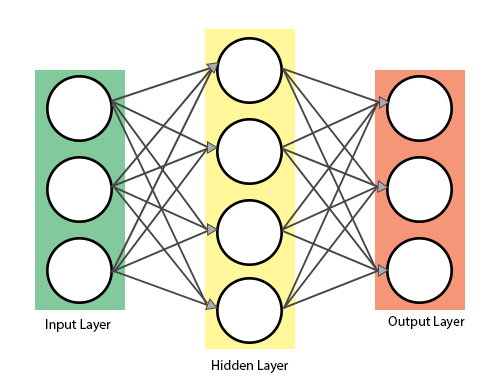
\includegraphics[width=0.6\textwidth]{common_layout}
    \caption{Common layout of a neural network.}%
    \label{fig:common_layout}
\end{figure}

% Include the basics of neural networks here - The biological aspect
% More explanation of the weights, and what their values can be.

\subsection{Deep Q Networks}

The main issue with using a tabular approach for keeping track of state-action
values is the number of required entries. As a more complex space needs to be
represented, the number of entries in the table would increase for every
possible combination of values. The newest approach to tackling the issue of
complex space environments is to use a neural network. The weights represent
what an expected value for a given state could be. The state is given as input
into the network and then the highest value output is chosen as an action to be
taken by the agent. The steps for running the network:

\begin{enumerate}
    \item A state is given as input into the network.
    \item The input is multiplied by the respective connected weights.
    \item The next layer is then given the input from the previous layer.
    \item The final output layer will return different values for each node in the layer.
    \item The node with the highest value represents the action to be taken.
    \item Once the action is taken, a reward value is recorded and used to update the network.
\end{enumerate}

The main difference between a Deep Q Network and a normal neural network is the
update function used. A Deep Q Network uses the loss function from the
Q-Learning algorithm to update the weights of the network. The loss function
provides a value of the target return and the predicted return. For example,
the agent could choose that in a certain state the best action would be the
third action with a value of 20. The agent takes the action and gets a returned
reward that is less. The network is then updated to return a lesser value for
that action next time the agent is in that state again. This is known as the TD
error:

\begin{align}
    TD Error = {(Q(s',a) - Q(s,a))}^{2}
\end{align}

The error is squared, as opposed to using the absolute value, to increase the
reduction level making the mistake more punishing on the network. This increase
speed at which the network converges to a better value return.

The update could be applied in real-time or at the end of every episode. When
using a real-time learning environment the agent is more likely to mistake an
action for being optimal from the first reward it gets. This makes the agent
tend to be more bias towards actions that get an immediate return and will not
allow the agent to see the possibilities of foreshadowing what could be a
better action in the long run. To avoid over fitting for a single environment,
the agent needs to be exposed to differing maps and states. Updating the
network at the end of each episode, may make the agent learn action pairs that
are incorrect and do not impact the reward factor. For example, the agent can
move left, which lets assume is correct, then go right and then left again.
This introduces a loop that the agent can get stuck in or an extra action step
that is unnecessary.

In order to avoid such an outcome, a discount factor $\gamma$ is used to reduce
the reward value for an incoming state. So the more steps an agent may take to
the reward, the lesser the reward value is. Once the agent takes an action,
based on the state given to the network, the reward is observed and used to
update the Q-Target. The Q-Target looks at the next states and checks which
action yields the highest value return. That value is then used to update the
current state in the network by using the TD Error.
% We need to state what "TD Error" is and how it is calculated.

\begin{align}
    QTarget = r + \gamma*Q(s',a)
\end{align}

The prediction made by the network is then
subtracted according to the TD Error equation. A learning rate is then
multiplied to the value. The final update value is:

\begin{align}
    Q(s,a) = Q(s,a) + \alpha (TDError)
\end{align}

The equation above is the same equation used in the Q-Learning algorithm. But
is implemented through the network with a gradient descent optimizer.
% Include a bit more explanation here of the basics of gradient decent and how
% it applies here.

\subsection{Convolutional Neural Networks}

\section{Challenges}
% Add more info here about the tech and the challenges it faces
% i.e. the problems in Reinforcement Learning as a whole

\section{Reinforcement Learning For Games}
% The earlier sections should cover the general tech,
% whereas this section will talk about it applied to games
% and the unique problems that raises.

\section{Existing Methods}
% This should then move on from the previous section
% to show how the outlined challenges are dealt with.

\section{Conclusion}
